\chapter{Modelo e Implementação}
\label{modelagem}

    \section{Modelo do sistema no \textit{framework} de atores}
        
        %modelo do programa para o teste com a jiga anterior mas flexivel para expansao
        % partimos do pressuposto da flexibilidade no setup de teste, para depois adequar ao setup atual.
        
        Foram determinados cinco módulos, conforme as competências de teste necessárias: comunicação com o módulo; leitura e validação do multímetro; teste de potência de RF; registro da execução de testes; e supervisão; Para cada um destes módulos, foi criada uma classe de ator. 
        
        Dessa forma, permitem-se diversos arranjos de software e flexibilidade de adaptação frente à configuração física de teste utilizada. Para o caso da configuração de teste atualmente utilizada e selecionada para este trabalho, foi elaborado um arranjo em topologia em estrela, conforme visto na figura \ref{fig:modelo}. A escolha desta topologia foi consequente às próprias limitações do \textit{Actor Framework} em termos de comunicação entre atores, que não permite a comunicação de atores que não sejam \textit{pais} ou \textit{filhos}. A principal vantagem desta topologia é o Controlador como entidade supervisora natural do sistema, para detecção e tratamento de atores em falha de execução.
        
        \begin{figure}
            \centering
            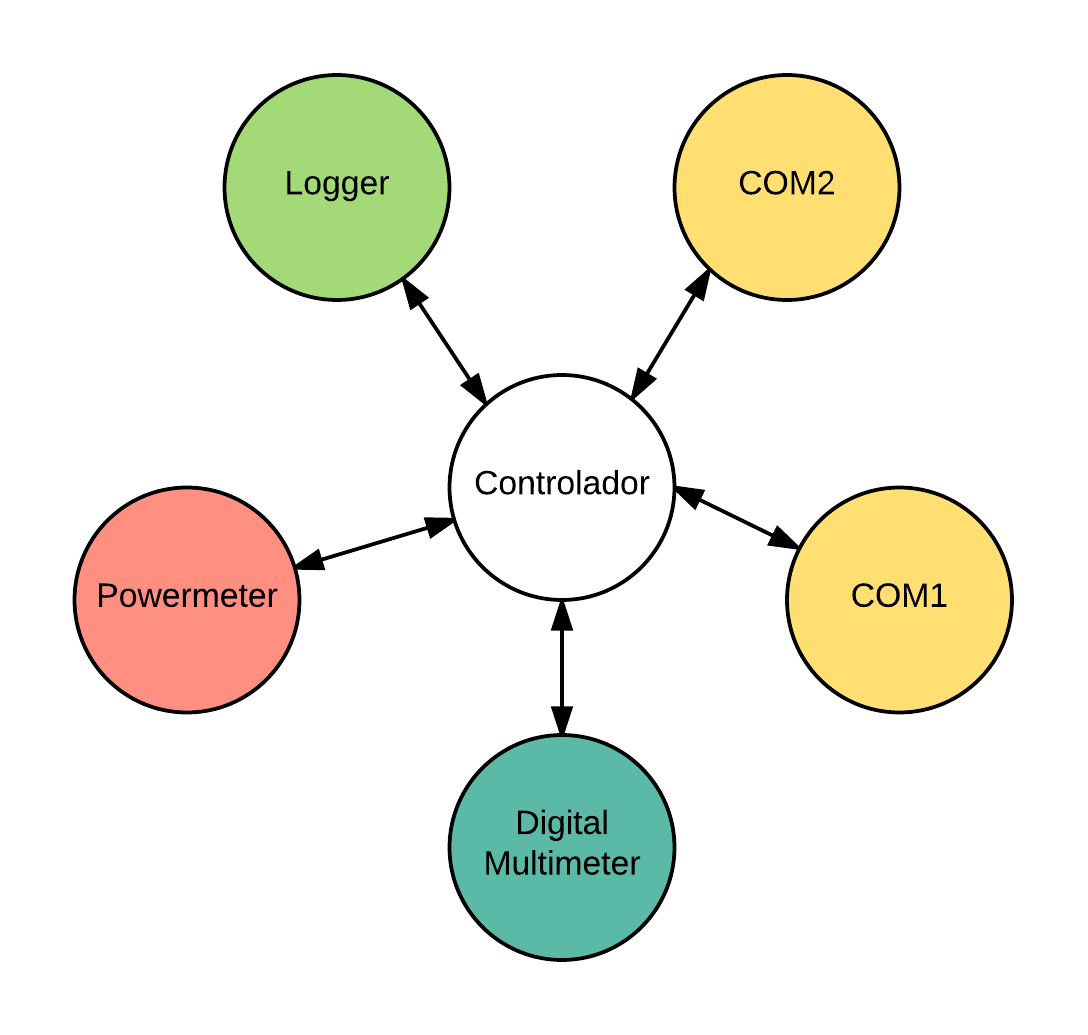
\includegraphics[width=0.9\linewidth]{fig/sistemmodel}
            \caption{Modelo do programa de teste reimplementado à partir do \textit{framework} de atores, e adequado para a jiga de teste legada}
            \label{fig:modelo}
        \end{figure}
            
        O Ator \texttt{ModCOM} é responsável pela comunicação com o DUT através de uma porta RS-232. Cumpre funções como enviar comandos de teste e verificar as respostas recebidas do dispositivo sob teste. Idealmente, este ator interpretaria trechos do roteiro da bateria de testes (em um arquivo xml), retornando o status da execução para o controlador. Todavia, devido ao curto prazo e simplificação do protótipo, a função de interpretação de roteiro foi deixada de lado. Dessa forma, o roteiro foi codificado diretamente no código fonte do programa, impossibilitando alterações de roteiro após a compilação.
        
        O ator \texttt{DMM} é incumbido pela leitura de dados do multímetro através da porta RS-232. A leitura dos pacotes do instrumento (figura \ref{fig:dmmprotocol}), sincronização e conversão de dados é realizada por ele, como também a interface de usuário para o operador do multímetro e a validação de medidas comparadas com a tabela de referências. 
        
        O registrador, ou \texttt{Logger}, é o ator responsável pelo registro da execução e resultados das baterias de testes. Dentre as suas incumbências estão: gerar um arquivo de registro completo do teste para fins de depuração e diagnóstico; gerar um arquivo de registro resumido para o controle de qualidade da produção e o envio direto dos registros para a base de dados de produção. 
                
        O Ator \texttt{Powermeter} detém o controle do medidor de potência RF, também referenciado como \textit{Powermeter}, responsável por toda a interface e configuração, e coleta de medições do NI 5680.
         
        O \texttt{Controller} ou controlador, como o próprio nome define, detém a responsabilidade sobre o fluxo de execução do programa, criando e destruindo os outros atores-módulos e fazendo a comunicação entre seus atores filhos. Além disso, detém a interface de usuário principal do programa.
        
        A relação entre as classes criadas com as classes base do \textit{framework} podem ser vistas no diagrama de classes UML da figura \ref{fig:classdiagram}. Nota-se que as mensagens entre atores possuem uma superclasse em comum e que, para cada ator, existem diversas classes de mensagens associadas a ele. Cada classe de mensagem se relaciona com um método interno do ator, funcionando como a interface pública deste ator. 
        Para melhor legibilidade, neste diagrama foram suprimidas as classes de mensagens, assim como muitas das VIs (\textit{Virtual Instruments}) das classes criadas.
        
            \begin{figure}
                \centering
                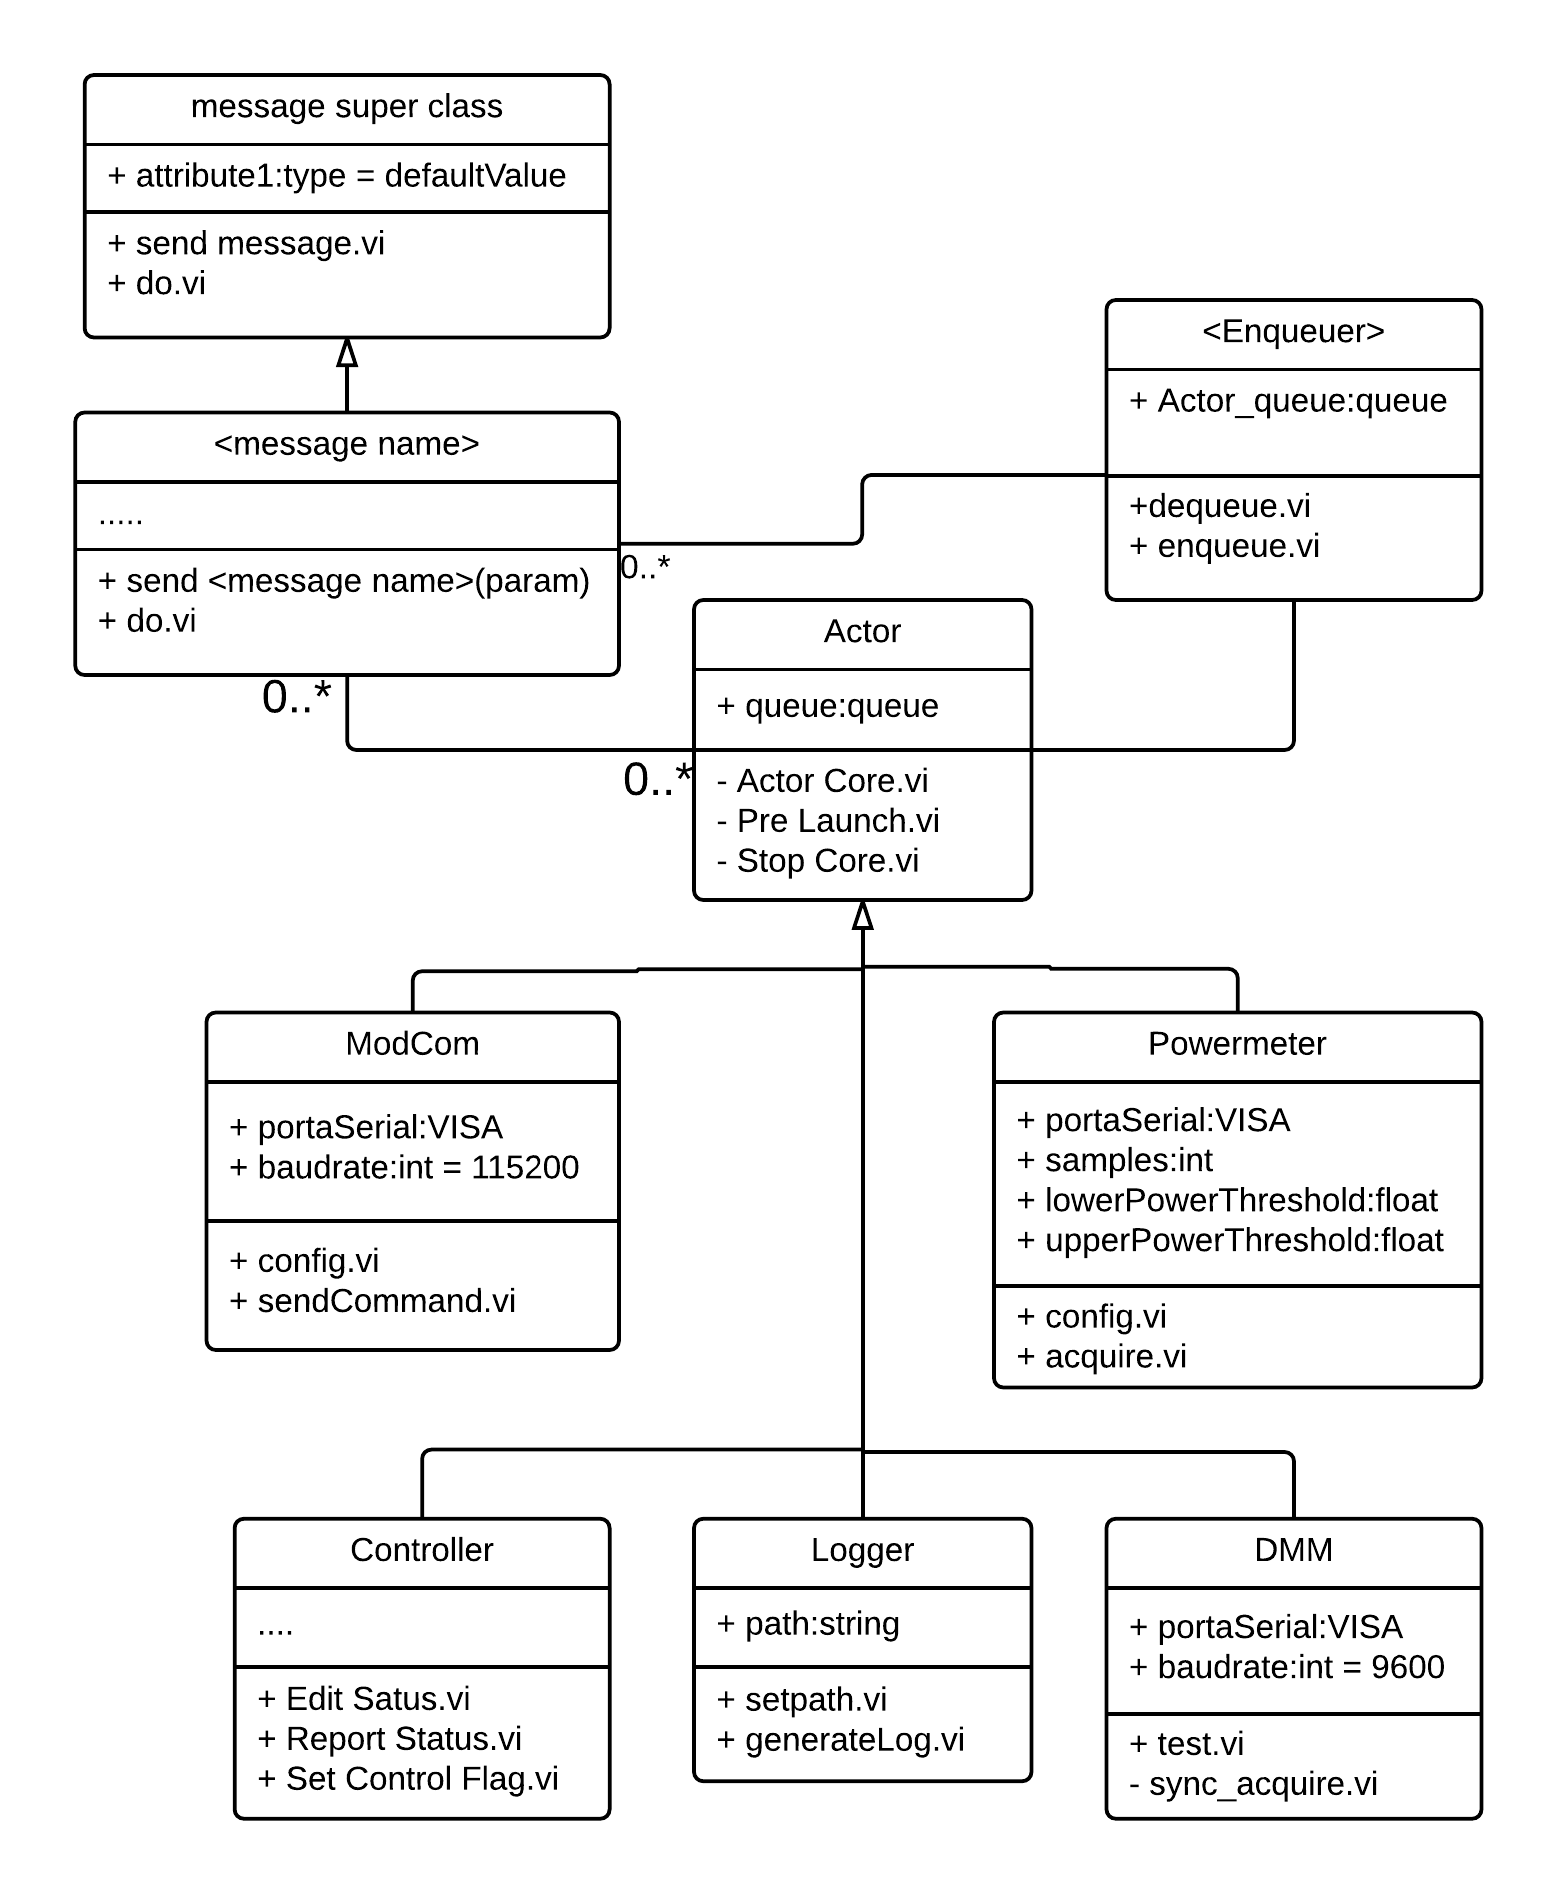
\includegraphics[width=1\linewidth]{model/class}
                \caption{Diagrama UML de classes simplificado retratando as classes do \textit{framework}, em conjunto com as classes de atores propostas e implementadas neste trabalho}
                \label{fig:classdiagram}
            \end{figure}
            
 
    \section{Implementação}
        
        Análoga à programação orientada a objetos, a implementação de um ator envolve a criação de métodos públicos e privados, sendo que todas as suas \textit{subVI} são privadas por padrão e podem ser acessíveis de maneira pública, se for criada uma classe de mensagem invocando-a. Dessa forma, o conjunto de classes de mensagens relacionadas àquele ator funciona como sua interface pública.
        
        Todas as implementações do módulos herdam da classes \texttt{actor} e \texttt{actor message} do \textit{framework} de atores. Todo ator tem que implementar a função \texttt{actor core.vi} para poder alterar o comportamento do ator. Como o próprio nome descreve, esta é a função núcleo do ator, responsável por sua inicialização e de seu tratador de mensagens. Também é possível e recomendável inserir nesta \texttt{vi} outras sub-rotinas, como, por exemplo, tratadores de eventos.    
        
        A interação dos atores filho com o \texttt{Controller} é realizada através de duas de suas classes de mensagens: \texttt{Set Control Flag}, que informa o status final de execução do teste e \texttt{Report Status}, que envia dados brutos do teste.
        
            
        \subsection{Ator de comunicação serial}
        \label{modcom}
        
            A comunicação serial em LabVIEW é realizada através de portas VISA (\textit{Virtual Instrument Software Architecture}) e são o padrão da National Instruments para configuração, programação, comunicação e depuração de sistemas de instrumentação. Dentro da VISA existe uma biblioteca própria para comunicação serial, que foi usada para criar as \textit{SubVI} base deste ator.
            
            O funcionamento deste ator é viabilizado pela \texttt{serialcore.vi}, a \textit{subVI} que envia comandos e captura respostas do dispositivo sob teste, como também confere respostas por padrões de \textit{strings}. É invocada diversas vezes por todos os outros métodos do ator. Esse funcionamento interno, assim como a relação do ator com agentes externos, estão ilustrados no diagrama da figura \ref{fig:diagserial}. 
            
            \begin{figure}
                \centering
                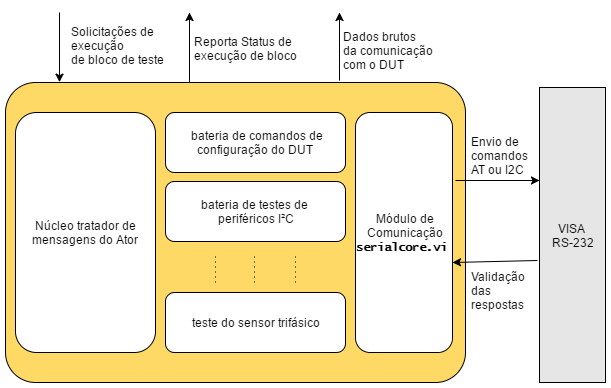
\includegraphics[width=1\linewidth]{fig/diag/blocoserial.png}
                \caption{Diagrama de blocos do \texttt{ModCOM}, ator de comunicação serial}
                \label{fig:diagserial}
            \end{figure}

            Todo o roteiro está escrito diretamente no código fonte do programa e as mensagens do \texttt{Controller} para o \texttt{ModCOM} consistem somente do pedido de execução de determinado bloco de teste interno. Devido à falta de generalização de sua interface,  este ator foi de longe aquele com o maior número de classes de mensagens. Para retornar dados brutos da comunicação com o módulo, o ator usa a mensagem \texttt{Report Status} do Controlador, que decide sobre a reexecução do bloco ou o término do teste.
            
            Por trabalhar com duas portas seriais, foram instanciados dois atores: para comunicar com o módulo por comandos AT e outro para acessar periféricos conectados no barramento  I$^{2}$C. 
            
            Apesar de não possuir uma interface gráfica de usuário própria, alguns métodos deste ator invocam as suas próprias. Destaca-se entre elas o teste de painel de LEDs, aonde foi empregado um painel esqueumórfico. Isso será mencionado na sessão \ref{ergo}, sobre ergonomia. 
        
            
            %De um ponto de vista externo o ator funciona da seguinte maneira:
            
            %Configura-se a porta através Após sua configuração - porta serial a ser usada, \textit{baudrate}, etc - o ator está pronto para comunicar com o módulo. Após receber do controlador o comando de testes para ser executado, o ator executa a rotina e reporta ao Controlador os dados de resposta, assim como o diagnóstico de aprovação ou reprovação.
            
            %Devido ao curto prazo dado ao projeto, nessa implementação inicial não foi implementado o interpretador para o padrão de roteiros utilizados no programa anterior. o que daria bastante flexibilidade à equipe para editar o roteiro conforme mudanças de \textit{firmware}, aplicação ou revisões de placa. Ao invés disso, todos os comandos são parte do código fonte do programa, situação conhecida como \textit{hardcoding}. No contexto desse projeto isto é considerado um antipadrão de projeto de software, já que assumimos que variável ambiental é constante. %todo cite anti patterns
            
        
        \subsection{Ator Multímetro}
            \label{dmmmodel}
            
            
            % falar da \texttt{sync_acquire vi} e como é a comunicação com ahrware e como é feita a Sincronização, tratamento do frame aquisiçaõ e envio de dados para a test.vi
            
            % falar da test.vi
            % como funciona o deboouncer e processo de validação de leitura do multimetro
            % GUI
            
            % que tipo de mensagens ele recebe do exterior.
            % configuração e acquisicao

            A implementação desta classe de ator, denominado \texttt{DMM}, começou pela função de aquisição e sincronia de \textit{frames}, acondicionados dentro da VI \texttt{sync\_acquire.vi}. Após a criação de uma interface de leitura serial do multímetro, foi criada uma máquina de estados para a sincronização dos \textit{frames}, já descritos pela figura \ref{fig:dmmprotocol}.
            
            
            Com a sincronização funcionando, desenvolveu-se um conjunto de SubVI para a conversão dos \textit{frames} em um \textit{cluster} com medidas e todas as informações adicionais que o multímetro fornece. Isso envolveu a decomposição dos \textit{frames}, conversão de código de sete segmentos em inteiros e associação de unidades de medida. 
            
            \texttt{test.vi} é a segunda VI fundamental deste ator, que checa as medidas recebidas de \texttt{sync\_acquire.vi} e provê uma interface gráfica de usuário para o operador de teste. A comunicação entre as duas VIs é feita através de uma fila. Sua interação dentro do ator é ilustrada pela figura \ref{fig:diagdmm}.
            
            \begin{figure}
                \centering
                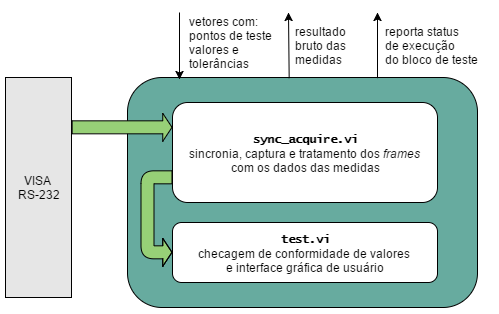
\includegraphics[width=0.9\linewidth]{fig/diag/diagdmm.png}
                \caption{Diagrama de blocos do \texttt{DMM}, ator de aquisição de medidas do multímetro digital}
                \label{fig:diagdmm}
            \end{figure}
            
            A checagem de medidas de \texttt{test.vi} é análoga a um algoritmo de \textit{debounce} de botão analógico e funciona em três estados:
            \begin{enumerate}
                \item Aguardar o valor da medida ficar dentro dos limites de tolerância para o valor de referência daquele ponto de medida. Exceção esperada: \textit{timeout}.
                \item Certificar-se de que a medida se mantém dentro da faixa de tolerância por um tempo especificado. Em caso de sucesso, ir para o estado 3 ou lançar uma exceção de erro de medida.
                \item Em caso de exceção, terminar o teste como reprovado ou permitir o reteste. Do contrário, passar para o próximo ponto de teste ou, se for o último ponto, aprovar a bateria de testes.
            \end{enumerate}

            Em caso do multímetro estar em um modo de operação incorreto, \texttt{test.vi} lança uma exceção e notifica o operador.  
            
            %colocar em erognomia?
            A interface gráfica de usuário (GUI) é exibida na figura \ref{fig:dmmfp}, onde o operador pode acompanhar as medições e qual ponto de teste deve deixar a ponta de prova. Também é notificado por sinais sonoros quando o ponto de teste é aprovado ou reprovado.
            
            \begin{figure}
                \centering
                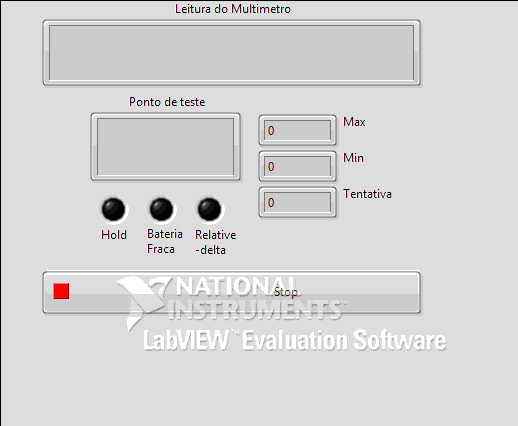
\includegraphics[width=0.8\linewidth]{lv/dmm/DMM_lvclass_DMM_UI_p}
                \caption{Painel da VI de aquisição de medidas do multímetro digital}
                \label{fig:dmmfp}
            \end{figure}
            
            Em termos de configuração, este ator precisa receber as seguintes informações: porta serial utilizada; tempo de estabilização de medida; número de tentativas; e o \textit{array} de pontos de teste com os seguintes atributos para cada ponto: \textit{limiar máximo; limiar mínimo; unidade de medida.}
            
            Assim como o ator \texttt{ModCOM}, o \texttt{DMM} utiliza-se do conjunto de mensagens do \texttt{Controller} para reportar o parecer final das medições, assim como os dados brutos de teste. 
            
            
        \subsection{Registrador de testes} 
            
            
            O gerenciador de registros, por sua baixa complexidade, foi implementado utilizando-se poucas VIs (figura \ref{fig:diaglog}). Este ator recebe do controlador de teste dois conjuntos de dados diferentes: os dados brutos da execução de teste e o cluster com os dados de teste resumidos. 
            A VI principal é \texttt{generateLog.vi}, que aglutina as conversões dos dados resumidos para JSON (\textit{JavaScript Object Notation}) e as dos dados brutos em documento de texto. 
            
              \begin{figure}
                \centering
                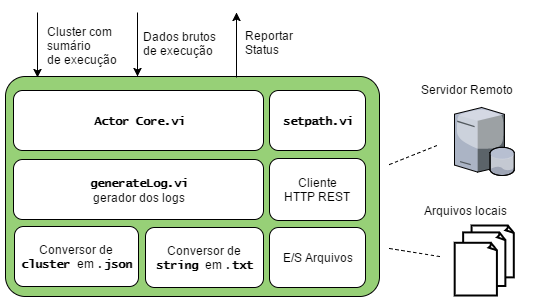
\includegraphics[width=0.9\linewidth]{fig/diag/diaglog.png}
                \caption{Diagrama de blocos do \texttt{logger}, ator atribuído de gerar arquivos de registro das baterias de testes}
                \label{fig:diaglog}
            \end{figure}
            
            
            % pertence à modelagem não?
            O registro com os dados brutos de execução contém o despejo da troca de mensagens pela serial, das medidas de tensão e potência, as exceções lançadas durante o teste e as métricas de desempenho. São dados necessários para a depuração e diagnóstico de problemas na placa e para melhor efetividade no retrabalho, sendo usados tanto em produção quanto em manutenção.
            
            A segunda classe de registro é um resumo estruturado da bateria de testes, o diagnóstico geral da placa e outras informações importantes para o controle e rastreamento dos produtos, requisito necessário para otimizações do processo produtivo, como também do próprio produto. Recebe o \textit{cluster} com os dados do DUT e resultados da bateria de teste e transforma em um objeto JSON.
            
            Quanto ao armazenamento, o ator suporta que seja feito tanto em servidor remoto, através de uma API REST, como também em pastas locais, através da biblioteca padrão de E/S de arquivos. O uso de arquivos locais é importante para o diagnóstico e depuração no local de fabricação, como também em situações sem conexão com a internet.
            
            
        \subsection{Sensoriamento de potência do \textit{front-end} RF}
        \label{pwmodel}
           
             
            % isso naõ é especificação?
            %Falar como a medida de potencia RF é realizada. Não é nenhum pouco conforme os padrões, mas serve para o propósito.
            
            %implementação
            O desenvolvimento deste ator foi simplificado com uso das bibliotecas e \textit{drivers} fornecidas pelo próprio fabricante. Estas bibliotecas possuem VIs de fácil utilização para configuração e aquisição de medidas e foram utilizadas na criação de \texttt{acquire.vi}, a VI principal deste ator. Esta VI recebe como entrada: frequência de medição, largura de banda, tamanho da janela de aquisição, número de amostras e limites máximo e mínimo de potência (em dBm). Seu funcionamento interno consiste em um laço simples de aquisição e comparação com a referência especificada. \texttt{config.vi} configura os dados internos do ator, como a porta USB utilizada. O ator pode ser visto na figura \ref{fig:diagpwmr}.
            
            \begin{figure}
                \centering
                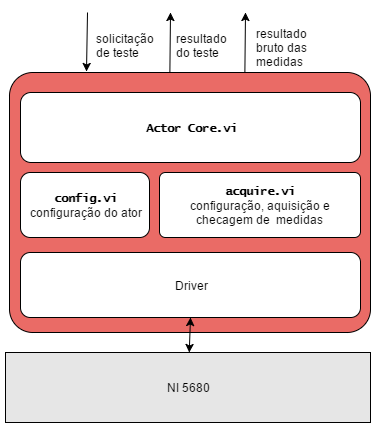
\includegraphics[width=0.7\linewidth]{fig/diag/diagpot.png}
                \caption{Diagrama de blocos do \texttt{PowerMeter}, ator de interface com o NI 5680}
                \label{fig:diagpwmr}
            \end{figure}
            
        \subsection{Controlador}
        
            % interface com outros atores - tipos de mensagem
            % funcionamento interno
            % como interage com o hardware
            % interface gráfica
            %extras    
            
            % Um geralzão dos módulos criados para fazer esse ator ser o que ele é. O que ele é? um ator de interface de usuário, watchdog e coordenador de atores filhos. 
            
            
            O \texttt{controller}, módulo de supervisão e controle de execução, é composto pelo módulo de inicialização de atores filhos e de dois laços acionados por eventos (figura \ref{fig:diagctrl}): a interface gráfica de usuário e o controle de fluxo de execução. 
            
            \begin{figure}
                \centering
                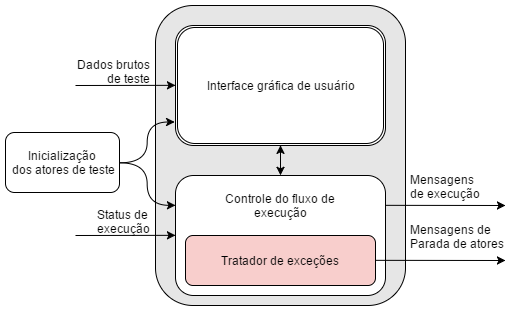
\includegraphics[width=0.9\linewidth]{fig/diag/diagctrl.png}
                \caption{Diagrama de blocos do \texttt{Controller}, ator supervisor}
                \label{fig:diagctrl}
            \end{figure}
            
            A escolha de uma estrutura orientada a eventos para o controle de fluxo de execução foi devido à sua sinergia com um sistema de atores e as trocas de mensagens entre eles. Dessa maneira, sempre que ele receber resposta de um ator filho, ele pode disparar outras mensagens de execução.
    
            O \texttt{Controller} possui o método \texttt{set control flag.vi} para que seus atores filhos relatem sucesso/falha de execução de subrotinas e baterias de testes. Para ser acessível às entidades externas ao ator, o método é exposto por uma classe de mensagem. Estas mensagens são usadas pelo bloco de controle de fluxo para alternar seu estado de execução e disparar outras mensagens para seus atores filhos.
            
            Outro método exposto por uma classe de mensagem é \texttt{report status.vi}, que é usada para transmitir ao \texttt{Controller} os registros de execução de teste e saída da porta serial. Todos os dados recebidos por estas mensagens vão para a interface de usuário, para depuração em tempo de execução e posteriormente, enviadas ao ator \texttt{Logger}.
            
            Seu tratador de exceção possui finalidades: parada, reinicialização e \textit{watchdog} de atores filhos e, como próprio sugere, tratamento de falhas de execução. Parte dele foi implementado a partir das funções de tratamento de erro do LabVIEW, do \textit{Actor Framework} e outras funções customizadas, especialmente para casos de desconfiguração de instrumentos de medida.
            
            A figura \ref{fig:cntrlpanel} expõe a interface de usuário do programa, que oferece ao usuário duas saídas de texto: despejo da comunicação serial, à esquerda, e o registro de execução das baterias de teste e medições, à direita. 
            
            \begin{figure}
                    \centering
                    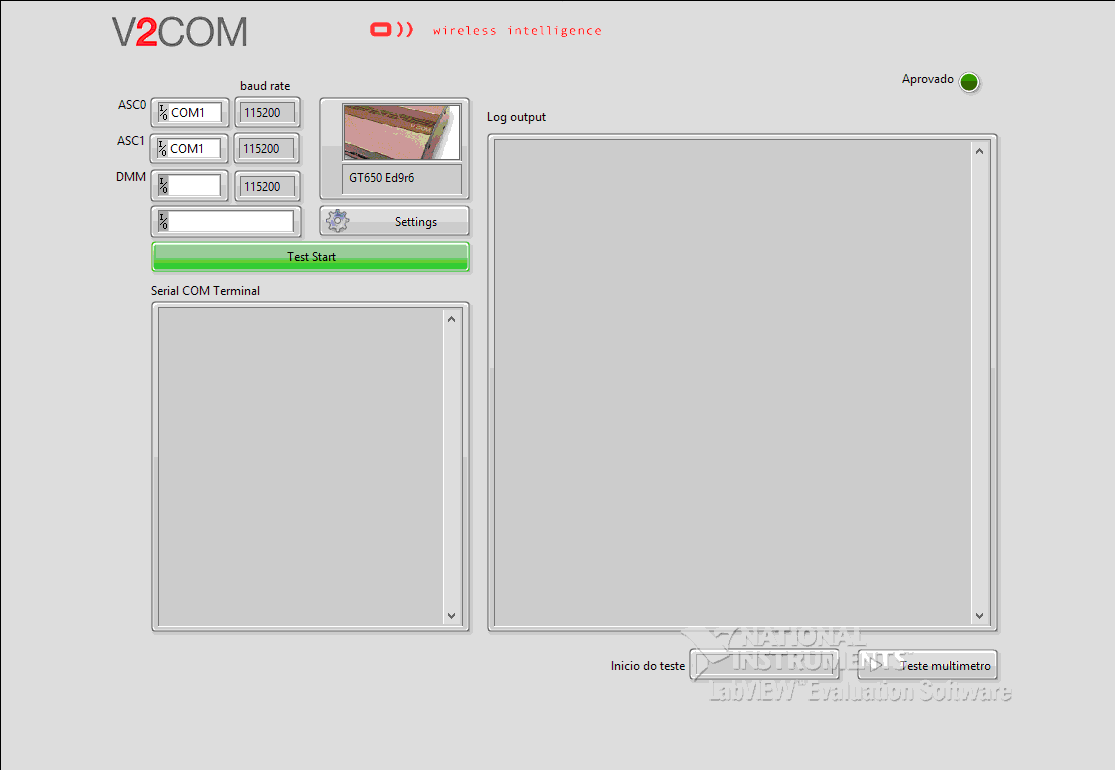
\includegraphics[width=0.8\linewidth]{lv/controler/Controller_lvclass_Actor_Corep}
                    \caption{Tela do painel principal de interface de usuário}
                    \label{fig:cntrlpanel}
            \end{figure}
        
        \subsection{Ergonomia}
        \label{ergo}
            
            % leds simulacro (sem uso do teclado
            % multimetro e a reduçaõ do uso do teclado
            % duas telas de depuracao
            
            A ergonomia no trabalho envolvido foi considerada durante todo o projeto e desenvolvimento do programa. As etapas de teste que envolvem a interação do trabalhador foram pensadas de forma a minimizar o esforço repetitivo e o desgaste do operador. No que confere à parte de software, o interesse é minimizar o uso do teclado e mouse, bem como a necessidade de dividir atenção visual entre o DUT e o monitor. As partes principais onde o operador precisa interagir com o software são: teste dos LEDs do painel, medição de tensões com o multímetro e testes de alimentação e bateria. 
            
            Para o teste do painel de LEDs do DUT foi criada uma GUI esqueumórfica (figura \ref{fig:modcomledp}) para facilitar a comparação com o painel real, agilizando e diminuindo erros no processo de verificação visual.
            
            \begin{figure}
                \centering
                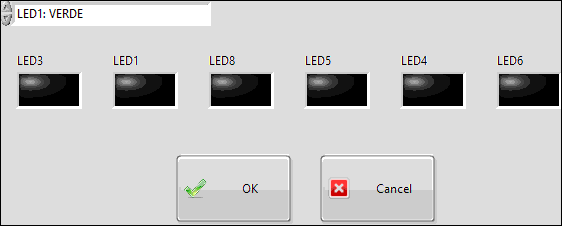
\includegraphics[width=0.8\linewidth]{lv/modcom/ModCOM_LED_popupp.png}
                \caption{Captura de tela do Painel de teste de led}
                \label{fig:modcomledp}
            \end{figure}
            
            Quanto às medições de tensões na placa, as mãos e atenção do operador se voltam para a DUT. Descuidos aqui podem causar erros ou, até mesmo, danos ao circuito. Em relação a isto, foi criado um \textit{debouncer} para validação das medidas, permitindo que o operador passe a ponteira pelos pontos de medição sem a necessidade de digitar ou interagir com o teclado. Além disso, referências sonoras foram criadas para os casos de aprovação, repetição ou reprovação de medição, de forma que a atenção visual do operador não precise desviar do DUT para o computador.
            
            Dentre as outras melhorias citam-se: a separação de uma tela dedicada somente ao registro da comunicação com o módulo para a melhor depuração; a redução de etapas de digitação por teclas simples ou mouse. 
        
\clearpage
